%
% File acl2012.tex
%
% Contact: Maggie Li (cswjli@comp.polyu.edu.hk), Michael White (mwhite@ling.osu.edu)
%%
%% Based on the style files for ACL2008 by Joakim Nivre and Noah Smith
%% and that of ACL2010 by Jing-Shin Chang and Philipp Koehn


\documentclass[11pt,letterpaper]{article}
\usepackage[letterpaper]{geometry}
\usepackage{acl2012}
\usepackage{times}
\usepackage{latexsym}
\usepackage{amsmath}
\usepackage{amsfonts}
 
\usepackage{multirow}
\usepackage{graphicx}
\usepackage{url}
\graphicspath{ {images/} }
\makeatletter
\newcommand{\@BIBLABEL}{\@emptybiblabel}
\newcommand{\@emptybiblabel}[1]{}
\makeatother
\usepackage[hidelinks]{hyperref}
\DeclareMathOperator*{\argmax}{arg\,max}
\setlength\titlebox{6.5cm}    % Expanding the titlebox

\title{Discrete Structured Representation Learning}

\author{Benjamin Striner \\
  {\tt bstriner@andrew.cmu.edu} \\}

\date{}

\begin{document}
\maketitle
\begin{abstract}
  Placeholder
\end{abstract}

\section{Introduction}

placeholder

\section{Factoring a joint distribution}

Let $A$ be a joint distribution matrix of two discrete variables $X$ and $Y$.

$$A_{i,j}=P(X=i, Y=j)$$

The entropy of the marginal distribution, $H(Y)$, measures the complexity of the data if only $Y$ is considered. In the case of a skipgram matrix, this is roughly the entropy of the unigram distribution.

\begin{align*}
f(x) &= -x \log(x) \\
P(Y=j) &= \sum_i A_{i, j} \\
H(Y) &=  \sum_j f(P(Y=j))
\end{align*}

The conditional entropy, $H(Y \mid X)$, measures the complexity of $Y$ if $X$ is known. A neural network trained given $X$ to predict $Y$ using cross-entropy loss will at best achieve this value. The conditional entropy is the joint probability times the log of the conditional probability, or alternatively the marginal probability times the entropy of the conditional distribution.

\setlength{\thinmuskip}{0mu}
\setlength{\medmuskip}{0mu}
\setlength{\thickmuskip}{0mu} 
$$H(Y \mid X)=\sum_{i,j} - P(X=i, Y=j) \log(P(Y=j \mid X=i)) $$
$$H(Y \mid X)= \sum_{i,j}  P(X=i) f(P(Y=j \mid X=i))$$

The function $f(x)=-x \log(x)$ is concave, therefore the entropy of a linear combination of distributions is greater than or equal to the linear combination of the entropy of the distributions. The entropy of the marginal distribution is greater than or equal to the conditional entropy.

\subsection{Continuous factoring}

The most common method of continuous factoring is to embed each input into some continuous representation. A neural network is used to parameterize an approximation ($\tilde{P}$) to the actual conditional distribution. The loss ($L$) is the expected negative log conditional likelihood. See, for example, \cite{DBLP:journals/corr/MikolovSCCD13} and \cite{DBLP:journals/corr/abs-1301-3781}. 

A simple version of this model is parameterized by embeddings ($x$), weights ($W$) and bias ($b$) and uses a softmax to squash the outputs.

$$ \tilde{P}(Y\mid X=i) = \operatorname{softmax}(x_i W+b)$$
$$ L(x,W,b) = -\sum^{i, j} P(Y=j,X=i) \log \tilde{P}(Y=j \mid X=i) $$
$$ L(x,W,b) = -\mathbb{E}_{[i \sim X, j \sim Y]} \log \tilde{P}(Y=j \mid X=i) $$

\subsection{Discrete factoring or clustering}

A common practice for producing discrete clusters is to train a neural network and then apply clustering techniques to the learned embeddings. In this paper, we examine how much information is actually retained by applying clustering to learned embeddings. We also examine methods to directly cluster with respect to a given loss function.

If examples in a dataset are clustered, the single output that minimizes the loss for a given cluster may be calculated analytically or iteratively. In the case of minimizing entropy, the analytic solution is straightforward.

$$\min_{\tilde{x}}\sum_i-x_i \log(\tilde{x_i}) = x$$

The expected negative log conditional likelihood is the conditional entropy of the combined distributions, analogous to the cross entropy loss in above discussion of continuous factoring. Similar approaches could be applied to more complicated neural networks, but discrete factorization of a conditional distribution is highly efficient and works well for analysis of the core optimization problem.

Let $C$ be an indicator matrix where $C_{j,i}$ indicates that $X=i$ should be encoded as $Z=j$. $C$ encodes the distribution $P(Z=z \mid X=x)$. $C$ is constrained to all $0$ except one and only one $1$ per column. The joint distribution matrix $B_{i,j}=P(Y=j,Z=i)$ is efficiently calculated using the dot product. 

$$P(Y=y,Z=z) = \sum_x P(Y=y,X=x) P(Z=z \mid X=x)$$
$$B = C A $$ 

If the inputs $X$ are encoded discretely into $Z$ where $Z$ is overfull, some information is lost.  The covariance matrix $B$ is a linear combination of rows of the matrix $A$ and therefore $H(Y|Z) \ge H(Y|X)$. 

By relaxing the constraints on $C$, we can create a parameterization that allows for gradient descent using the conditional entropy $H(Y\mid Z)$ as the loss. A simple parameterization
is $C=\operatorname{softmax}(W)$. If the softmax is fully saturated, each row will be assigned to one and only one cluster. At initialization, each row is assigned to a random mixture of clusters. The softmax ensures that $C$ may be vallidly interpreted as $P(Z \mid X)$. By the concavity of $f$, we predict that the model will tend towards saturation. A mixture of distributions will have a higher entropy than the component distributions.

$$ L(W) = - \sum_{x,y} P(X=x, Y=y) \log( P(Y=y \mid Z=z)) $$

\subsection{Hierarchical clustering}

The simplest discrete structured encoding is a binary tree. The address of a node in a binary tree of depth $d$ may be represented as a vector of length $d$ containing only zeros and ones. A complete binary tree will contain $2^d$ leaves at the base of the tree and will ideally achieve similar performance to models using $2^d$ flat clusters.

A reasonable loss for hierarchical clusters is the weighted sum of the conditional entropy of the clusters at each depth in the tree. In the spirit of the Bellman equation, an exponential series is a reasonable choice of weighting. Let $C_d \in [0,1]^{(2^d, \lvert Y \rvert)}$ be the cluster membership indicator at each depth in the tree.

$$ L = \sum_d \beta ^ d  H(Y \mid C_d) $$

Intuitively, one is optimizing a weighted sum of how much information is available given the depth ($d$) of the tree or how many bits of the representation are provided. The parameter $\beta$ controls the balance of having more information available early or better accuracy given more of the tree. This model attempts to pack more information into the early bits and remaining differentiation into the later bits. The meaning of the later bits is dependent on the earlier bits but the converse is not true.

We parameterize clusters at at the bottom layer of the tree $C_d$. We can then infer the membership of clusters at previous layers $C_0,...,C_{d-1}$ by summing leaves into parent nodes. We can then calculate the weighted loss over tree depth as described above.

\section{Results}

We built a skipgram matrix from the Brown corpus as a simple distribution so we could focus on aspects of the optimization problem. [corpus specifics]

The entropy of the marginal distribution created from our matrix is 5.913 and the conditional entropy of the matrix is 5.326. Any reasonable factorization of the matrix should result in performance somewhere between those two values.

\subsection{Random clustering}

We assessed an initial baseline by randomly and uniformly assigning words to clusters. As the number of clusters increased, the conditional entropy of the output given the cluster decreased (Figure \ref{f:random}). Given two clusters, the mean conditional entropy is 5.9109 ($\sigma=0.0004$). Given 1024 clusters, the mean conditional entropy is 5.5664 ($\sigma=0.0018$).

\begin{figure}
  \caption{Random uniform clustering}
\label{f:random}
  \centering
    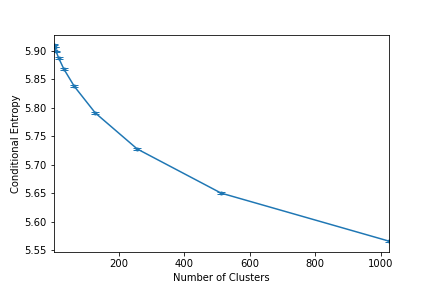
\includegraphics[width=0.5\textwidth]{random.png}
\end{figure}

\subsection{Post-mortem clustering}

We trained unregularized continuous skipgram models varying the number of hidden units and found that performance asymptotically approached the analytically calculated conditional entropy (Figure \ref{f:baseline}). 

\begin{figure}
  \caption{Continuous skipgram model}
\label{f:baseline}
  \centering
    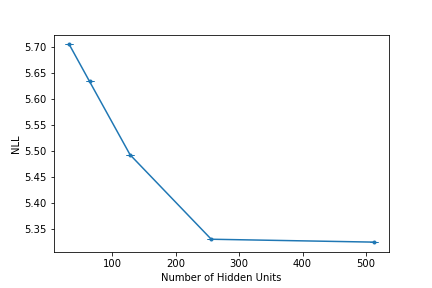
\includegraphics[width=0.5\textwidth]{baseline.png}
\end{figure}

We additionally trained models with l1 and l2 regularization. We performed clustering on each model to examine how regularization and the number of hidden units affect the quality of post-mortem clustering. 

We performed binary GMM clustering (Figure \ref{f:bgmm}) and k-means clustering (Figure \ref{f:km}). The best performance of any post-mortem binary clustering trial was 5.89231.

\begin{figure}
  \caption{Binary GMM clustering}
\label{f:bgmm}
  \centering
    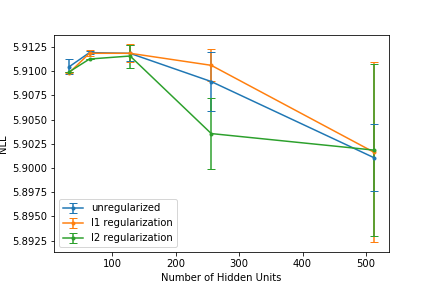
\includegraphics[width=0.5\textwidth]{binary_gmm.png}
\end{figure}


\begin{figure}
  \caption{Binary K-means clustering}
\label{f:bkm}
  \centering
    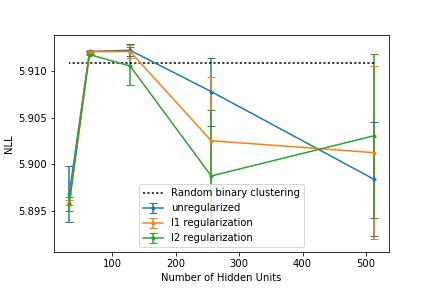
\includegraphics[width=0.5\textwidth]{binary_km.png}
\end{figure}

We also clustered into 1024 groups using GMM clustering (Figure \ref{f:fgmm}) and k-means clustering (Figure \ref{f:fkm}). The best performance of any post-mortem clustering with $k=1024$ was 5.59504.

\begin{figure}
  \caption{GMM clustering ($k=1024$)}
\label{f:fgmm}
  \centering
    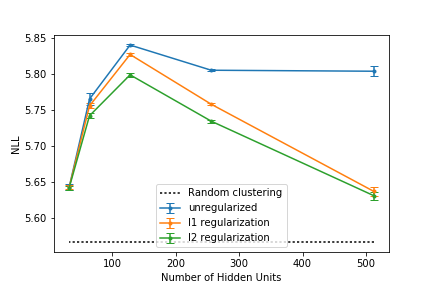
\includegraphics[width=0.5\textwidth]{flat_gmm.png}
\end{figure}


\begin{figure}
  \caption{K-means clustering ($k=1024$)}
\label{f:fkm}
  \centering
    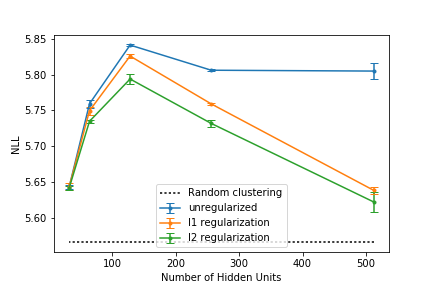
\includegraphics[width=0.5\textwidth]{flat_km.png}
\end{figure}

\subsection{Proposed flat models}

We trained our model to discretely factor the matrix into 2 clusters of words. The mean conditional entropy of the resulting matrix was 5.8856 ($\sigma=4.4e-08$).

We also trained an unregularized model to discretely factor the matrix into 1024 clusters of words. The mean conditional entropy of the resulting clusters was 5.5480 ($\sigma=0.00078$). The model accomplished this performance without utilizing all clusters, so we knew that improvements were possible. The average utilization (out of 1024 clusters) was 809.4 ($\sigma=4.8$).

We trained models with varying regularizer weights to determine the effect regularizer choice and weight has on conditional entropy and utilization. We experimented with the uniform prior regularizer (Figure \ref{f:fb}), exclusive lasso regularizer (Figure \ref{f:fel}), square root of the exclusive lasso (Figure \ref{f:fels}), L1 (Figure \ref{f:fl1}), and L2 (Figure \ref{f:fl2}) regularizers. The best performing model using the uniform prior regularizer was 5.5175 and the best using the exclusive lasso regularizer was 5.5166.

\begin{figure}
  \caption{Uniform Prior Regularization ($k=1024$)}
\label{f:fb}
  \centering
    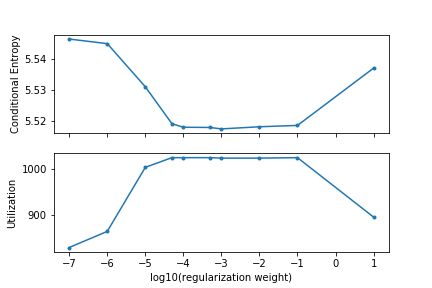
\includegraphics[width=0.5\textwidth]{skipgram_flat_b.png}
\end{figure}
\begin{figure}
  \caption{Exclusive Lasso Regularization ($k=1024$)}
\label{f:fel}
  \centering
    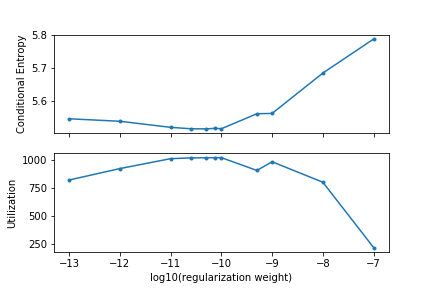
\includegraphics[width=0.5\textwidth]{skipgram_flat_el.png}
\end{figure}
\begin{figure}
  \caption{Sqrt Exclusive Lasso Regularization ($k=1024$)}
\label{f:fels}
  \centering
    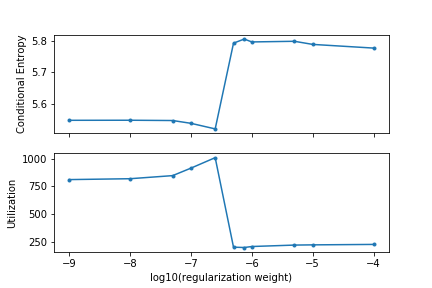
\includegraphics[width=0.5\textwidth]{skipgram_flat_els.png}
\end{figure}
\begin{figure}
  \caption{L1 Regularization ($k=1024$)}
\label{f:fl1}
  \centering
    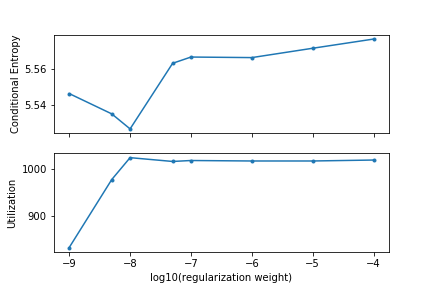
\includegraphics[width=0.5\textwidth]{skipgram_flat_l1.png}
\end{figure}
\begin{figure}
  \caption{L2 Regularization ($k=1024$)}
\label{f:fl2}
  \centering
    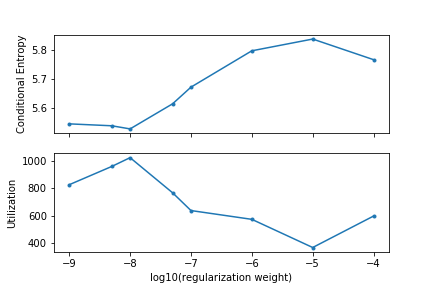
\includegraphics[width=0.5\textwidth]{skipgram_flat_l2.png}
\end{figure}

\subsection{Proposed binary tree models}

We trained binary trees of depth 10 so as to compare to our flat models of 1024 ($2^{10}$) clusters.

We trained our binary tree model varying $\beta$ to analyze the effect of the Bellman decay parameter (Figure \ref{f:beta}). 

\begin{figure}
  \caption{Effect of Beta Hyperparameter}
\label{f:beta}
  \centering
    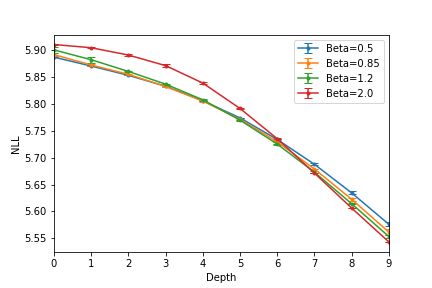
\includegraphics[width=0.5\textwidth]{skipgram_tree.png}
\end{figure}
\bibliography{tacl}
\bibliographystyle{acl2012}

\end{document}



